\section{Wektory styczne}

\textbf{Oznaczenia z analizy matematycznej:}
\begin{itemize}
  \item dla gładkiej funkcji $f:(a, b)\to\R^n$ takiej, że $f=(f_1,...,f_n)$ i dla $t\in (a, b)$ pochodną nazywamy wektor
    $$f'(t)=\frac{\partial f}{\partial t}(t)=\begin{pmatrix}f_1'(t)\\f_2'(t)\\...\\f_n'(t)\end{pmatrix}$$
  \item dla gładkiego odwzorowania $f:U\to\R^m$, $U\subseteq \R^n$ i $p\in U$ oznaczamy macierz pierwszych pochodnych cząstkowych w punkcie $p$ przez $D_pf$. Dokładniej, jeśli $f=(f_1,...,f_m)$ i $f_i:U\to\R^m$ są wszystkie gładkie, to
    $$D_pf=\begin{pmatrix}\frac{\partial f_1}{\partial x_1}(p) & \frac{\partial f_1}{\partial x_2}(p) & \hdots & \frac{\partial f_1}{\partial x_n}(p)\\
      \vdots & \vdots & \vdots & \vdots\\
    \frac{\partial f_m}{\partial x_1}(p) & \frac{\partial f_m}{\partial x_2}(p) & \hdots & \frac{\partial f_m}{\partial x_n}(p) \end{pmatrix}$$
    Tym samym symbolem oznaczamy też odwzorowanie liniowe $\R^n\to\R^m$ zadane tą macierzą (różniczka $f$ w $p$).
\end{itemize}

\subsection{Przestrzeń styczna - definicja kinematyczna}

Przestrzeń styczną będziemy definiować przez styczność krzywych gładkich.
\marginpar[]{J.M. Lee definiuje przestrzeń styczną przy pomocy derywacji oraz przedstawia możliwość użycia m.in. kiełków funkcji gładkich}

Niech $M$ będzie gładką rozmaitością. \acc[b]{Krzywą gładką} na $M$ nazywamy gładkie odwzorowanie $c:(a, b)\to M$. O krzywej gładkiej $c$ takiej, że $c(t_0)=p$ mówimy, że jest \acc[i]{zbazowana w $p$}. Zbiór par $(c, t_0)$ krzywych zbazowanych w $p$ oznaczamy ${\color{green}C_pM}$.

\begin{definition}[styczność krzywych w mapie]
  Niech $\phi:U\to \R^n$ będzie mapą wokół $p$. Krzywe $(c_1,t_1)$ i $(c_2, t_2)$ zbazowane w $p$ są do siebie styczne w mapie $(U,\phi)$ jeśli $(\phi\circ c_1)'(t_1)=(\phi\circ c_2)'(t_2)$.
\end{definition}

\begin{lemma}[styczność w jednej mapie $\iff$ styczność w każdej mapie]
  Jeżeli $(c_1,t_1),(c_2,t_2)\in C_pM$ są styczne w mapie $(U,\phi)$ wokół $p$, to są też styczne w dowolnej innej mapie $(W, \psi)$ wokół $p$ (zgodnej z $(U, \phi)$.
\end{lemma}

\begin{proof}
  \begin{align*}
    (\psi\circ c_1)'(t_1)&=[(\psi\circ\phi^{-1})\circ(\phi\circ c_1)(t_1)]'=D_{\phi(p)}(\psi\circ\phi^{-1})\circ [(\phi\circ c_1)'(t_1)]=\\
                         &=D_{\phi(p)}(\psi\circ\phi^{-1})[(\phi\circ c_2)'(t_2)]=[(\psi\circ\phi^{-1})\circ(\phi\circ c_2)(t_2)]'\\
                         &=(\psi\circ c_2)'(t_2)
  \end{align*}
\end{proof}

\begin{definition}[styczność krzywych]
  Krzywe $(c_1,t_1),(c_2,t_2)\in C_pM$ są styczne, jeżeli są styczne w pewnej (równoważnie każdej) mapie wokół $p$.
\end{definition}

Relacja styczności krzywych jest relacją równoważności na $C_pM$, bo jest zwrotnia, symetryczna i przechodnia ($(\phi\circ c_1)'(t_1)=(\phi\circ c_2)'(t_2)\text{ i }(\phi\circ c_2)'(t_2)=(\phi\circ c_3)'(t_3)\implies(\phi\circ c_1)'(t_1)=(\phi\circ c_3)'(t_3)$).

\begin{definition}[przestrzeń styczna]
  \important{Przestrzenią styczną} do $M$ w punkcie $p$ nazywamy zbiór klas abstrakcji relacji styczności krzywych zbazowanych w $p$
  $$T_pM:=C_pM/stycznosc$$
  Klasę abstrakcji krzywej $(c, t_0)\in C_pM$ oznaczamy przez $[c, t_0]$ lub $c'(t_0)$. Elementy przestrzeni $T_pM$ nazywamy \acc[b]{wektorami stycznymi} do $M$ w punkcie $p$.
\end{definition}

\subsection{Struktura wektorowa przestrzeni $T_pM$}

Dla mapy $\phi:U\to \R^n$ wokół $p\in M$ określamy dwa odwzorowania:
\marginpar{Odwzorowanie $\phi_p^*$ jest dobrze określone z definicji $T_pM$ (wszystkie krzywe z jednej klasy abstrakcji mają tę samą pochodną w jednej mapie).}
\begin{align*}
  &\phi_p^*:T_pM\to\R^n\quad\; \phi_p^*([c, t_0])=(\phi\circ c)'(t_0)\in \R^n\\
  &\lambda_{\phi,p}:\R^n\to T_pM\quad \lambda_{\phi,p}(v)=[c_v, 0]
\end{align*}
gdzie $c_v(t)=\phi^{-1}(\phi(p)+tv)$. 

\begin{lemma}
  $\phi^*_p\circ\lambda_{\phi, p}=id_{\R^n}$ oraz $\lambda_{\phi, p}\circ\phi_p^*=id_{T_pM}$, czyli $\phi_p^*$ i $\lambda_{\phi,p}$ są one wzajemnie jednoznacze i do siebie odwrotne.
\end{lemma}

\begin{proof}
  Niech $v\in\R^n$, wtedy
  \begin{align*}
    \phi_p^*\circ\lambda_{\phi, p}(v)&=\phi^*_p([c_v, 0])=(\phi\circ c_v)'(0)=\frac{d}{dt}_{{\scriptstyle|t=0}}\phi(\phi^{-1}(\phi(p)+t\cdot v))=\\
                                     &=\frac{d}{dt}_{{\scriptstyle|t=0}}(\phi(p)+tv)=v &\checkmark
  \end{align*}

  Niech $[c, t_0]\in T_pM$
  $$\lambda_{\phi, p}\circ\phi_p^*([c, t_0])=\lambda_{\phi, p}((\phi\circ c)'(t_0))=[c_{(\phi\circ c)'(t_0)}, 0]$$
  gdzie $c_{(\phi\circ c)'(t_0)}(t)=\phi^{-1}(\phi(p)+t(\phi\circ c)'(t_0))$. W mapie $\phi$ zachodzi więc:
  $$(\phi\circ c_{(\phi\circ c)(t_0)})'(0)=\frac{d}{dt}_{{\scriptstyle|t=0}}[\phi(p)+t\cdot(\phi\circ c)'(t_0)]=(\phi\circ c)'(t_0)$$
  W takim razie $(c, t_0)$ i $(c_{(\phi\circ c)'(t_0)}, 0)$ są krzywymi stycznymi i mamy $[c, t_0]=[(c_{(\phi\circ c)'(t_0)}, 0]$ i w takim razie $\lambda_{\phi, p}\circ\phi_p^*([c, t_0])=[c, t_0]\quad\checkmark$.
\end{proof}

\begin{fact}[struktura przestrzeni wektorowej na przestrzeni stycznej]\label{przestrzen styczna jest wektorowa}
Na przestrzeni stycznej $T_pM$ istnieje dokładnie jedna struktura przestrzeni wektorowej, dla której odwzorowania $\phi_p^*$ oraz $\lambda_{\phi, p}$ dla wszystkich map $\phi$ wokół $p$ są liniowymi izomorfizmami. 
\end{fact}

Struktura ta jest zadana przez operacje dodawania wektorów i mnożenia ich przez skalary następująco:
\begin{itemize}
  \item dla $X, Y\in T_pM$: $X+Y:=\lambda_{\phi, p}(\phi^*_p(X)+\phi^*_p(Y))$ (suma w środku jest sumą w $\R^n$)
  \item dla $a\in\R$: $a\cdot X:=\lambda_{\phi, p}(a\cdot \phi_p^*(X))$ (mnożenie przez skalar w $\R^n$).
\end{itemize}

\begin{proof} Struktura przestrzeni wektorowej musi być przeniesiona z $\R^n$ przez $\lambda_{\phi, p}$. Wystarczy więc uzasadnić, że dla różnych map $\phi,\psi$ wokół $p$ przeniesione z $\R^n$ na $T_pM$ struktury liniowe pokrywają się, to znaczy złożenie odwzorowań

\begin{center}\begin{tikzcd}
\R^n\arrow[r, "\lambda_{\phi, p}"]&T_pM\arrow[r, "\psi_p^*=\lambda_{\psi,p^{-1}}"]&\R^n
\end{tikzcd}\end{center} 

jest liniowe.

\begin{align*}
  \psi_p^*\circ\lambda_{\phi,p}(v)&=\psi_p^*([c_v,0])=(\psi\circ c_v)'(0)=\frac{d}{dt}_{{\scriptstyle|t=0}}\psi\circ\phi^{-1}(\phi(p)+tv)=\\
                                  &=D_{\phi(p)}(\psi\circ\phi^{-1})[\frac{d}{dt}_{{\scriptstyle|t=0}}(\phi(p)+tv)]=D_{\phi(p)}(\psi\circ\phi^{-1})(v)
\end{align*}
Przekształcenie $\psi_p^*\circ\lambda_{\phi, p}$ pokrywa się z działaniem macierzy $D_{\phi(p)}(\psi\circ\phi^{-1})$, a więc jest liniowe.

\end{proof}

O odwzorowaniu $\phi_p^*:T_pM\to\R^n$ można myśleć jak o "mapie" dla $T_pM$ stowarzyszonej z mapą $\phi$ otoczenia punktu $p$. W tej mapie działania na wektorach z $T_pM$ sprowadzają się do zwykłych działań na wektorach w $\R^n$.

\phantomsection\label{mapa na T_pR}
\textbf{Przykład:}
\begin{itemize}
  \item Dla $M=\R^n$ mamy wyróżnioną mapę $\phi:M=\R^n\to \R^n$, $\phi=id_{\R^n}$. Dla każdego $p\in M$ mapa ta, poprzez $\phi_p^*=(id_{\R^n})^*$ kanonicznie utożsamia $T_p\R^n$ z $\R^n$.
  \item Analogiczna sytuacja zachodzi z $M=U\subseteq\R^n$ otwartego podzbioru i $p\in U$, gdzie inkluzja $i:U\to\R^n$ jest traktowana jako mapa.
\end{itemize}

\begin{wrapfigure}{r}{5.5cm}
\centering
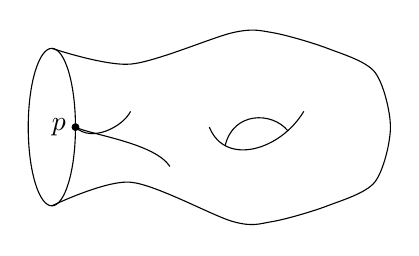
\begin{tikzpicture}
  %\draw plot [smooth cycle] coordinates {(0, 0) (-0.4, -0.5) (-0.5, -1) (-0.4, -1.7) (-0.2, -2) (0, -1.9) (0.4, -1.5) (0.5, -1.1) (0.55, -0.7) (0.4, -0.3)};
  \draw plot [smooth] coordinates {(0, 0) (1, -0.2) (2.3, 0.2) (2.8, 0.2) (3.5, 0) (4.1, -0.3) (4.3, -1) (4.1, -1.7) (3.5, -2) (2.8, -2.2) (2.3, -2.2) (1, -1.7) (0, -2)};
  \draw (0, -1) ellipse(0.3 and 1);
  \draw (2, -1)..controls(2.2, -1.5)and(2.9, -1.3)..(3.2, -0.8);
  \draw (2.2, -1.24)..controls(2.3, -0.8)and(2.8, -0.8)..(3, -1.05);
  \filldraw (0.3, -1) circle (1.2pt) node [left] {$p$};
  \draw (0.3, -1)..controls(0.5, -1.2)and(0.9, -1)..(1, -0.8);
  \draw (0.3, -1)..controls(0.5, -1.1)and(1.3, -1.2)..(1.5, -1.5);
\end{tikzpicture}
\end{wrapfigure}
Dla rozmaitości $M$ z brzegiem i $p\in \partial M$ dopuszczamy dodatkowo krzywe gładkie $c:[t_0, b)\to M $ oraz $c:(a, t_0[\to M$ takie, że $c(t_0)=p$ oraz pary $(c, t_0)$ jako elementy $C_pM$. Inaczej dla niektórych "kierunków" wektorów nie istniałyby odpowiednie krzywe reprezentujące te wektory. Styczność na $T_pM$ określa się potem w sposób analogiczny jak dla rozmaitości bez brzegu.
\medskip

Wektory styczne do $M=\R^n$ (lub $U\subseteq \R^n$) w punkcie $p$ odpowiadające wektorom bazowym $e_1=(1,0,0,...,0), e_2=(0, 1, 0, ..., 0) ,...,e_n=(0,0,0,...,1)$ oznaczamy przez $\frac{\partial}{\partial x_1}(p),\frac{\partial}{\partial x_2}(p),...,\frac{\partial}{\partial x_n}(p)$. Tworzą one bazę $T_p\R^n$ ($T_pU$), zaś dowolny wektor z $T_p\R^n$ ($T_pU$) ma postać $\sum_{i=1}^na_i\frac{\partial}{\partial x_i}(p)$.
\marginpar[]{Sens wprowadzenia takiego oznaczenia stanie się jasny później, gdy wektory utożsamimy z tzw. derywacjami}[0cm]

Analogicznie, dla dowolnej rozmaitości $M$ i $p\in M$ oraz mapy $\phi$ wokół $p$ przeciwobraz przez $\phi_p^*:T_pM\to\R^n$ wersorów $e_1,...,e_n$ oznaczamy:
$$\color{green}(\phi_p^*)^{-1}(e_i)=\frac{\partial}{\partial\phi_i}(p).$$
Elementy te tworzą bazę $T_pM$ i dowolny wektor z $T_pM$ ma postać $\sum a_i\frac{\partial}{\partial\phi_i}(p)$.

\begin{figure}[h]
  \begin{illustration}
    \draw(2, 2)rectangle(4, 4) node [above] {$\R^n$};
    \draw[->] (3, 1.8)--(3, 4.2);
    \draw[->] (1.8, 3)--(4.2, 3);
    \draw[->, very thick] (3, 3)--(3, 3.7) node [left] {$e_2$};
    \draw[->, very thick] (3, 3)--(3.7, 3) node [below] {$e_1$};

    \draw(-2, 0) arc (180:270:1);
    \draw(-1, 0) arc (220:280:1);
    \draw(-0.9, -0.1) arc (110:30:0.6);
    \draw(-1, -1) arc (90:45:2);
    \draw(0.41, -1.578) arc (220:300:1.5);
    \draw(2.3,-1.915) arc (300:400:1.2);
    \draw(2.626, -0.104) arc (50:90:3);

    \draw plot [smooth, tension=1] coordinates {(0.7, 0.6) (0, 0.7)  (-1.4,1) (-2, 0)};

    \draw plot[domain=0:350,smooth cycle, xshift=1.5cm, yshift=-0.8cm] (\x:0.5+rnd*0.2);
    \node at (0.8, -1.3) {$U$};

    \draw (0.5, -1.8)--(3, -1.5)--(2.5, 0.2)--(0, -0.1) node [above] {$T_pM$} -- cycle;
    \draw[very thick, ->] (1.5, -0.8)--(1.05, 0.3);
    \draw[very thick, ->] (1.5, -0.8)--(3, -0.55);
    
    \draw[<-] (4, -2)--(4, -4);
    \draw[->] (3, -3)--(5, -3) node [above] {$\R^n$};


    \draw plot[domain=0:350,smooth cycle, xshift=4cm, yshift=-3cm] (\x:0.4+rnd*0.2);

    \draw[->] (2.3, -1)..controls(3, -1)and(3.5, -1.8)..(3.7, -2.5) node [midway, above] {$\phi$};

    \draw[->] (2.7, 0)..controls(3, -0.1)and(4, 0.2)..(3.5, 1.8) node [midway, right] {$\phi_p^*$};
    
    \draw (1.1, -0.1)..controls(0.5, -0.2)and(0, 0.5)..(-0.5, 1.7) node [above] {$\frac{\partial}{\partial\phi_2}(p)$};
    \draw (2.9, -0.6)..controls(3.5, -0.5)and(4.5, -0.3)..(5, 0.5) node [above] {$\frac{\partial}{\partial\phi_1}(p)$};
  \end{illustration}
\end{figure}

\subsection{Różniczka}

Rozważmy funkcję gładką $f:M\to N$ i $p\in M,f(p)=q\in N$. Dla krzywej zbalansowanej $(c, t_0)\in C_pM$ mamy $(f\circ c, t_0)\in C_qN$.

\begin{lemma}[krzywe styczne po przejściu przez f:M->N są nadal styczne] \label{styczne po przejsciach}
  Jeżeli $(c_1, t_1),(c_2, t_2)\in C_pM$ są styczne, to $(f\circ c_1, t_1),(f\circ c_2, t_2)\in C_qN$ też są styczne
\end{lemma}

\begin{proof}
  Niech $\phi$ będzie mapą wokół $p$, $\phi:U\to\R^m$, zaś $\psi$ mapą wokół $q$,

  $\psi:W\to\R^n$
  \begin{align*}(\psi\circ f\circ c_1)'(t_1)&=[(\psi\circ f\circ\phi^{-1})\circ(\phi\circ c_1)]'(t_1)=D_{\phi(p)}(\psi\circ f\circ \phi^{-1})\cdot[(\phi\circ c_1)'(t_1)]=\\
  &=D_{\phi(p)}(\psi\circ f\circ\phi^{-1})\cdot[(\phi\circ c_2)'(t_2)]=[(\psi\circ f\circ\phi^{-1})\circ(\phi\circ c_2)]'(t_2)=\\
  &=(\psi\circ f\circ c_2)'(t_2)\end{align*}
  Zatem krzywe $(f\circ c_1, t_1)$ i $(f\circ c_2, t_2)$ są styczne.
\end{proof}

\begin{definition}[różniczka] \important{Różniczką} $f$ w punkcie $p$ nazywamy odwzorowanie $df_p:T_pM\to T_{f(p)}N$ określone przez $df_p([c, t_0])=[f\circ c, t_0]$.
\end{definition}

Odwzorowanie różniczkowe jest dobrze określone na mocy Lematu \ref{styczne po przejsciach}.

\begin{lemma}[df jest odwzorowaniem liniowym]
  $df_p:T_pM\to T_{f(p)}N$ jest odwzorowaniem liniowym.
\end{lemma}

\begin{proof}
  Wystarczy sprawdzić, że odwzorowanie

  \begin{center}\begin{tikzcd}
    \R^m\arrow[r, "\lambda_{\phi,p}"] & T_pM \arrow[r, "df_p"] & T_{f(p)}N\arrow[r, "\psi_{f(p)}^*"] & \R^n
  \end{tikzcd}\end{center}
  jest liniowe (analogicznie jak przy dowodzie \ref{przestrzen styczna jest wektorowa}). 
  \begin{align*}
    \psi_{f(p)}\circ df_p\circ\lambda_{\phi, p}(v)&=\psi_{f(p)}^*\circ df_p([c_v, 0])=\psi_{f(p)}^*([f\circ c_v, 0])=\\
                                                  &=(\psi\circ f\circ c_v)'(0)=[(\psi\circ f\circ \phi^{-1})\circ(\phi\circ c_v)]'(0)=\\
                                                  &=D_{\phi(p)}(\psi\circ f\circ\phi^{-1})\cdot[(\phi\circ c_v)'(0)]=\\
                                                  &=D_{\phi(p)}(\psi\circ f\circ \phi^{-1})[v]
  \end{align*}
  jest to przekształcenie zadane macierzą, a więc liniowe.
\end{proof}

Dla gładkiej funkcji $f:M\to N$ odwzorowanie $df_p:T_pM\to T_{f(p)}N$ wyznaczyliśmy w mapach $\phi$ wokół $p$ i $\psi$ wokół $f(p)$ jako
$$\psi_{f(p)}^*df_p\lambda_{\phi, p}(p)=D_{\phi(p)}(\psi f\phi^{-1})(v).$$
Stąd, odwzorowanie $df_p$ w bazach $\{\frac{\partial}{\partial\phi_i}(p)\}$ w $T_pM$ i $\{\frac{\partial}{\partial\psi_j}(p)\}$ w $T_{f(p)}N$ zapisuje się macierzą
$$D_{\phi(p)}(\psi f\phi^{-1})=\left(\frac{\partial(\psi f\phi^{-1})_i}{\partial x_j}(\phi(p))\right)_{ij}$$
$$df_p\left[\sum a_i\frac{\partial}{\partial\phi_i}(p)\right]=\sum_i\left[\sum_j\frac{\partial(\psi f\phi^{-1})}{\partial x_j}(\phi(p))\cdot a_j\right]\frac{\partial}{\partial\psi_i}(f(p)) $$

\textbf{Przykłady:}
\begin{itemize}
  \item Niech $\phi:U\to\R^n$ będzie mapą wokół $p\in M$. Możemy ją potraktować jako gładkie odwzorowanie między dwiema rozmaitościami. Wówczas różniczka $d\phi_p:\underset{{\scriptstyle =T_pM}}{T_pU}\to T_{\phi(p)}\R^n$ jest wówna odwzorowaniu "mapowemu" $\phi_p^*:T_pM\to\R^n$.

    \begin{proof}
      Niech $[c, t_0]\in T_pM$, wtedy
      $$d\phi_p([c, t_0])=[\phi\circ c, t_0]\in T_{\phi(p)}\R^n$$
      Mapę $(id_{\R^n})^*_{\phi(p)}:T_{\phi(p)}\R^n\to \R^n$ \hyperref[mapa na T_pR]{kanonicznie utożsamiliśmy} z $id_{\R^n}$, stąd też
      $$d\phi_p([c, t_0])=(id_{\R^n}\circ\phi\circ c)'(t_0)=(\phi\circ c)'(t_0),$$
      a z kolei
      $$\phi_p^*([c, t_0])=(\phi\circ c)'(t_0)\in\R^n$$
      z definicji tego odwzorowania.
    \end{proof}
  \item Dla gładkiej krzywej $c:(a, b)\to M$ oraz $t_0\in (a, b)$, różniczka $dc_{t_0}:T_{t_0}(a, b)\to T_{c(t_0)}M$ jest jedynym przekształceniem liniowym, które wersor z $\R\cong T_{t_0}(a, b)$ przekształca na wersor $[c, t_0]=c'(t_0)\in T_{c(t_0)}M$.
  \item Rozważmy gładką funkcję $f:M\to \R$ i $p\in M$. Różniczka $df_p:T_pM\to T_{f(p)}\R\cong \R$ jest funkcjonałem liniowym na $T_pM$. 
\end{itemize}

\begin{definition}[pochodna kierunkowa]
Dla funkcji $f:M\to\R$ możemy wybrać wektor styczny $X=[c, t_0]\in T_pM$ i zdefiniować \important{pochodną kierunkową} funkcji $f$ w kierunku wektora $X$: 
$$\color{blue}Xf=df_p(X)=df_p([c, t_0])=(f\circ c)'(t_0).$$
\end{definition}

Pochodna kierunkowa ma następujące własności:
\begin{itemize}
  \item $X(f+g)=Xf+Xg$
  \item $X(f\cdot g)=g(p)\cdot Xf+f(p)\cdot Xg$ (\acc[i]{reguła Leibniza})
    \begin{proof}
      \begin{align*}
        X(f\cdot g)&=[(f\cdot g)\circ c]'(t_0)=[(f\circ c)\cdot(g\circ c)]'(t_0)=\\
                            &=(f\circ c)'(t_0)\cdot(g\circ c)(t_0)+(f\circ c)(t_0)\cdot(g\circ c)'(t_0)=\\
                            &=Xf\cdot g(p)+f(p)\cdot Xg
      \end{align*}
    \end{proof}
  \item dla $a\in \R$ $(aX)f=a(Xf)$
  \item jeśli $X, Y\in T_pM$, to $(X+Y)f=Xf+Yf$
    \begin{proof}
      $$(X+Y)f=df_p(X+Y)=df_p(X)+df_p(Y)=Xf+Yf$$
    \end{proof}
\end{itemize}

\textbf{Przykłady:}
\begin{itemize}
  \item \marginpar{Stąd oznaczenie $\frac{\partial}{\partial x_i}(p)$, które ma charakter operatorowy związany z działaniem tego wektora na funkcjach $f_n$}Jeśli $X=\frac{\partial}{\partial x_i}(p)\in T_p\R^n$ i mamy gładką funkcję $f:\R^n\to\R$, to wówczas $Xf=\frac{\partial f}{\partial x_i}(p)$. 
  \item \marginpar{$\frac{\partial f}{\partial\phi_i}$ jest to $i$-ta pochodna cząstkowa $f$ w mapie $\phi$ w punkcie $p$}Jeśli $X=\frac{\partial}{\partial\phi_i}(p)\in T_pM$ i $f:M\to\R$ jest funkcją gładką, to oznaczamy 
    $$Xf=\frac{\partial(f\phi^{-1})}{\partial x_i}(\phi(p)=:\frac{\partial f}{\partial \phi_i}(p)$$
  \item Podobnie jak wyżej, jeśli $X=\sum a_i\frac{\partial}{\partial \phi_i}(p)$, to
    $$Xf=\sum a_i\frac{\partial f}{\partial\phi_i}(p)=\sum a_i\frac{\partial f\circ\phi^{-1}}{\partial x_i}(\phi(p))$$
\end{itemize}
